% !TEX root = main.tex
\subsubsection*{Process 입출력 규모의 영향}
State는 3개, 입력 합계는 $(320,30,231)$, 출력 합계는 $(300,30,261)$로 고정한다.
질량 손실률 6.25\%, 추가 탄소 30, WASTE 생성률 0\%이며 모든 출력은 ELIGIBLE이다.
출력 $N=1$에서 입력 $M$을, 입력 $M=2$에서 출력 $N$을 각각 늘렸다.
\begin{center}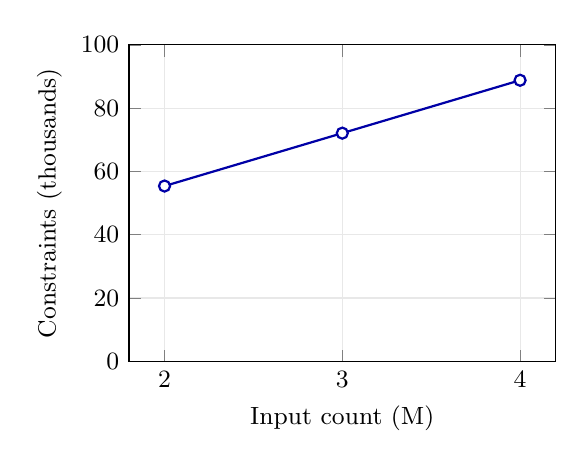
\begin{tikzpicture}\begin{axis}[width=7cm,height=5.6cm,grid=major,major grid style={gray!18},scaled ticks=false,tick label style={font=\small},label style={font=\small},xlabel={Input count (M)},ylabel={Constraints (thousands)},xtick={2,3,4},ymin=0,ymax=100]
            \addplot+[thick,mark options={fill=white},color=blue!65!black,mark=*] coordinates {(2,55.402) (3,72.116) (4,88.832)};
        \end{axis}\end{tikzpicture}\hspace{0.25cm}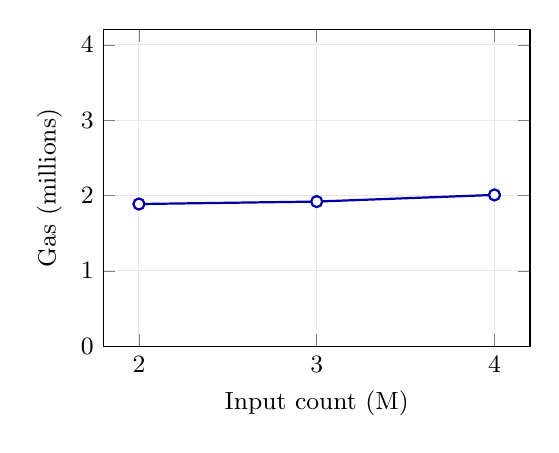
\begin{tikzpicture}\begin{axis}[width=7cm,height=5.6cm,grid=major,major grid style={gray!18},scaled ticks=false,tick label style={font=\small},label style={font=\small},xlabel={Input count (M)},ylabel={Gas (millions)},xtick={2,3,4},ymin=0,ymax=4.2]
            \addplot+[thick,mark options={fill=white},color=blue!65!black,mark=*] coordinates {(2,1.887935) (3,1.920611) (4,2.009039)};
        \end{axis}\end{tikzpicture}\end{center}
\begin{center}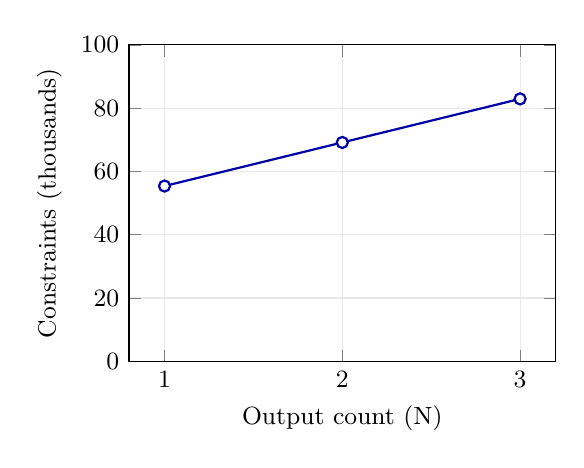
\begin{tikzpicture}\begin{axis}[width=7cm,height=5.6cm,grid=major,major grid style={gray!18},scaled ticks=false,tick label style={font=\small},label style={font=\small},xlabel={Output count (N)},ylabel={Constraints (thousands)},xtick={1,2,3},ymin=0,ymax=100]
            \addplot+[thick,mark options={fill=white},color=blue!65!black,mark=*] coordinates {(1,55.402) (2,69.172) (3,82.944)};
        \end{axis}\end{tikzpicture}\hspace{0.25cm}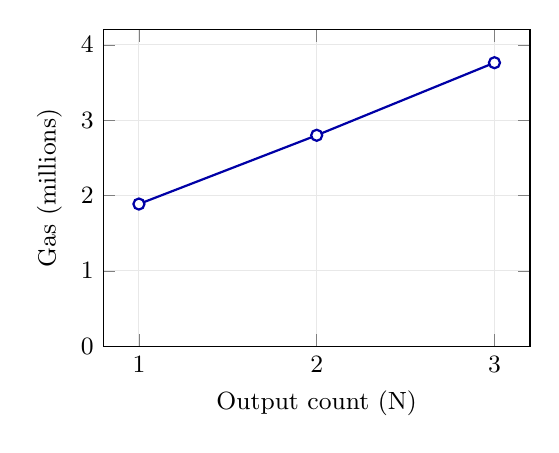
\begin{tikzpicture}\begin{axis}[width=7cm,height=5.6cm,grid=major,major grid style={gray!18},scaled ticks=false,tick label style={font=\small},label style={font=\small},xlabel={Output count (N)},ylabel={Gas (millions)},xtick={1,2,3},ymin=0,ymax=4.2]
            \addplot+[thick,mark options={fill=white},color=blue!65!black,mark=*] coordinates {(1,1.887935) (2,2.800596) (3,3.763779)};
        \end{axis}\end{tikzpicture}\end{center}
{\small 그림 4. Audit on Process의 독립 입력·출력 증가. 같은 지표의 축 범위를 맞췄다.}\par
\begin{center}\small\setlength{\tabcolsep}{6pt}
    \textbf{표 8. Process 입출력 개수별 비용}\par\smallskip
    \begin{tabular}{@{}lrrr@{}}\toprule
        \textbf{M} & \textbf{N} & \textbf{Constraints} & \textbf{Gas} \\ \midrule
        2          & 1          & 55,402               & 1,887,935    \\
        3          & 1          & 72,116               & 1,920,611    \\
        4          & 1          & 88,832               & 2,009,039    \\
        2          & 2          & 69,172               & 2,800,596    \\
        2          & 3          & 82,944               & 3,763,779    \\
        \bottomrule\end{tabular}\end{center}

공식 측정은 조건별 1회다. 개별 case의 입력·출력 합계와 실제 receipt가 원자료에 보존되어 있으며, 이번 정리에서도 합계를 대조했다.
입력 2→4에서 Constraints는 60.34\%, Gas는 6.41\% 증가했다. 출력 1→3에서는 각각 49.71\%, 99.36\% 증가했다.
이는 측정한 형상과 상태에서의 관측이며, 일반적인 선형 법칙은 아니다.

기준 $2\to1$의 Gas 1,887,935는 기본 Event 실험의 1,866,617과 다르다.
기본 실험은 전체 lifecycle 중간의 Process이고, 보충 실험은 별도 Entry로 준비한 원장에서 실행했다.
보충 Ledger는 arity 허용 조건도 확장했다. 차이 21,318을 특정 연산 하나의 효과로 단정하거나 두 수치를 통일하지 않는다.
    {\small 근거: process-independent.json, 각 case의 inputs·outputs·receipt, verification-after.json [D6].}\par

